\section{Bases de x86-64}
A compiler ultimately has to emit machine code, so the bottom of the pipeline
has to be understood before the top of it means anything. This chapter is the
target language: the x86-64 \textbf{instruction set architecture}
(\textit{Instruction Set Architecture}, ISA), the GAS syntax in which it is
written by hand, and enough of Linux's system-call interface to get a program
to produce visible output without any library at all.

\subsection{Modèle Simplifié}
\subsubsection{Le Mémoire d'un Ordinateur}
Le modèle d'un ordinateur used in this course has two kinds of storage:
\textbf{Registres} (\textit{registers}), and \textbf{RAM} (\textit{Random Access Memory}). 

\begin{figure}[h!]
  \centering
  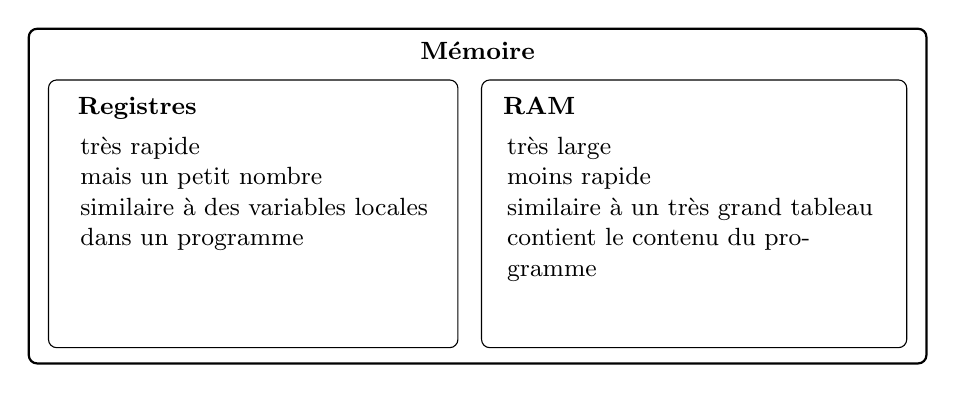
\begin{tikzpicture}[font=\small]
    \draw[rounded corners=3pt, thick] (-0.25,-0.25) rectangle (11.15,4);
    \node[anchor=north] at (5.45,3.95) {\textbf{Mémoire}};
    \draw[rounded corners=3pt] (0,-0.05) rectangle (5.2,3.35);
    \node[anchor=north west] at (0.25,3.25) {\textbf{Registres}};
    \node[anchor=north west, text width=4.55cm] at (0.28,2.75)
      {très rapide\\ mais un petit nombre\\ similaire à des variables locales dans un programme};
    \draw[rounded corners=3pt] (5.5,-0.05) rectangle (10.9,3.35);
    \node[anchor=north west] at (5.65,3.25) {\textbf{RAM}};
    \node[anchor=north west, text width=4.7cm] at (5.7,2.75)
      {très large\\ moins rapide\\ similaire à un très grand tableau\\ contient le contenu du programme};
  \end{tikzpicture}
\end{figure}

\subsubsection{Le Programme}
\begin{definition}[Programme]
  Un \textbf{programme} ce sont des instructions dans la RAM à une adresse.
\end{definition}
Un registre spécial --- \verb|%rip| en x86-64, le \textbf{pointeur d'instruction}
(\textit{instruction pointer}) --- contient l'adresse de l'instruction courante.\\

Chaque instruction peut:
\begin{itemize}
  \item lire ou écrire des registres;
  \item lire ou écrire une case de la RAM; ou
  \item faire un appel à l'OS (\textbf{syscall}).
\end{itemize}

\begin{remark}
  Ce modèle ne gère pas : disque, écran, clavier, souris, etc. Tous les effets
  du programme sur le monde extérieur passent par l'OS.
\end{remark}

\begin{example}[Factorial of $R_0$ in the abstract model]
  With registers $R_0$, $R_1$ and $R_{IP}$, the factorial of $R_0$ is computed
  by the following six instructions. Only the writes to $R_{IP}$ make control
  flow.

  \medskip
  \centering
  \begin{tabular}{c l l}
    \toprule
    Instruction & Effect & \\
    \midrule
    0 & $R_1 = 1$, \quad $R_{IP} = R_{IP} + 1$ & $R_{IP}$ = next instruction \\
    1 & if $R_0 = 0$ then $R_{IP} = 5$, else $R_{IP} = R_{IP} + 1$ & conditional jump \\
    2 & $R_1 = R_0 \times R_1$, \quad $R_{IP} = R_{IP} + 1$ & \\
    3 & $R_0 = R_0 - 1$, \quad $R_{IP} = R_{IP} + 1$ & \\
    4 & $R_{IP} = 1$ & unconditional jump \\
    5 & rest of the program, or end & \\
    \bottomrule
  \end{tabular}
\end{example}

\subsection{L'Assembleur}
\begin{definition}[Assembleur]
  \textbf{Assembleur} est le langage lisible dans lequel on écrit du code
  traduit ensuite vers du binaire. Aussi: Le programme qui fait cette traduction.
\end{definition}
\subsubsection{Instruction Set Architecture}
\begin{definition}[Instruction Set Architecture (ISA)]
  \textbf{ISA} est l'ensemble des instructions qu'un processeur peut exécuter,
  et la manière dont elles sont codées en binaire.
\end{definition}

The assembleur depends on the ISA but there may be multiple syntaxes for
the same ISA.
\begin{example}[Intel vs AT\&T/GAS syntax]
  The Intel syntax is used in the Intel manuals and in the Visual Studio IDE.
  The AT\&T/GAS syntax is used by the GNU Assembler (GAS) and by GCC.
  Between the two syntaxes the order of operands is reversed: Intel writes
  \verb|mov rax, rbx| while GAS writes \verb|mov %rbx, %rax|.
\end{example}

\subsubsection{Le Format Binaire}
\begin{definition}[Processus]
  Un \textbf{processus} (\textit{process}) est un programme en cours d'exécution. Il peut
  aussi être vu comme un état de la mémoire: le contenu des registres et de la RAM.
\end{definition}
\begin{definition}[Exécutable]
  Un \textbf{exécutable} (\textit{executable}) est un fichier qui contient un
  programme et les informations nécessaires pour que l'OS le charge en mémoire
  et lancer le processus correspondant.
\end{definition}
There are several formats for exécutables:
\begin{itemize}
  \item \textbf{Executable and Linking Format} (ELF) under Unix, except Mac;
  \item \textbf{Portable Executable} under Windows;
  \item \textbf{Mach-O} or PEF under Mac.
\end{itemize}

\begin{remark}
  In this course, we study the ELF format, used in Linux, with the x86-64 ISA
  and the GAS syntax.
\end{remark}

\subsection{La mémoire en x86-64}
\subsubsection{Les Registres Généraux}
x86-64 exposes sixteen 64-bit registres généraux:
\begin{center}
  \begin{tabular}{l l @{\qquad\qquad} l l}
    \toprule
    \multicolumn{2}{c}{Compute registers} & \multicolumn{2}{c}{Pointer registers} \\
    Name & ``Historical'' function & Name & ``Historical'' function \\
    \midrule
    \verb|rax| & Accumulator & \verb|rsi| & Source index \\
    \verb|rbx| & Base        & \verb|rdi| & Destination index \\
    \verb|rcx| & Counter     & \verb|rsp| & Stack Pointer \\
    \verb|rdx| & Data        & \verb|rbp| & Base Pointer \\
    \bottomrule
  \end{tabular}
\end{center}

\noindent along with 8 x86-64 registers with no pre-established function,
\verb|r8| through \verb|r15|.

Each register can be addressed at four widths by their \textbf{sous-registres}
(\textit{subregisters}), each a \emph{part of} the same physical register. e.g.
Writing \verb|%al| leaves the upper 56 bits of \verb|%rax| untouched.

\begin{center}
  \begin{tabular}{l l l l l}
    \toprule
    $b_0 \dots b_{63}$ & $b_0 \dots b_{31}$ & $b_0 \dots b_{15}$ & $b_8 \dots b_{15}$ & $b_0 \dots b_7$ \\
    Quad (q) & Double (d/l) & Word (w) & Byte (b) & Byte \\
    \midrule
    \verb|rax| & \verb|eax| & \verb|ax| & \verb|ah| & \verb|al| \\
    \verb|rbx| & \verb|ebx| & \verb|bx| & \verb|bh| & \verb|bl| \\
    \verb|rcx| & \verb|ecx| & \verb|cx| & \verb|ch| & \verb|cl| \\
    \verb|rdx| & \verb|edx| & \verb|dx| & \verb|dh| & \verb|dl| \\
    \verb|rsi| & \verb|esi| & \verb|si| &            & \verb|sil| \\
    \verb|rdi| & \verb|edi| & \verb|di| &            & \verb|dil| \\
    \verb|rsp| & \verb|esp| & \verb|sp| &            & \verb|spl| \\
    \verb|rbp| & \verb|ebp| & \verb|bp| &            & \verb|bpl| \\
    \verb|r8|  & \verb|r8d| & \verb|r8w| &           & \verb|r8b| \\
    \bottomrule
  \end{tabular}
\end{center}

The \verb|r8| row is the pattern for all eight registers:
\verb|r|$n$\verb|d|, \verb|r|$n$\verb|w|, \verb|r|$n$\verb|b|.

\begin{remark}
  The suffix letters \verb|q|, \verb|l|, \verb|w|, \verb|b| can also be
  appended to instructions to state how many bytes the operation touches.
\end{remark}

\subsubsection{Adressage Virtuel}
Memory is seen as an array of $2^{64}$ bytes. Each process has its own
translation from the address to memory, which is not necessarily on the RAM.
This translation is provided by the OS, depending on its state of paging.
\begin{figure}[h!]
  \centering
  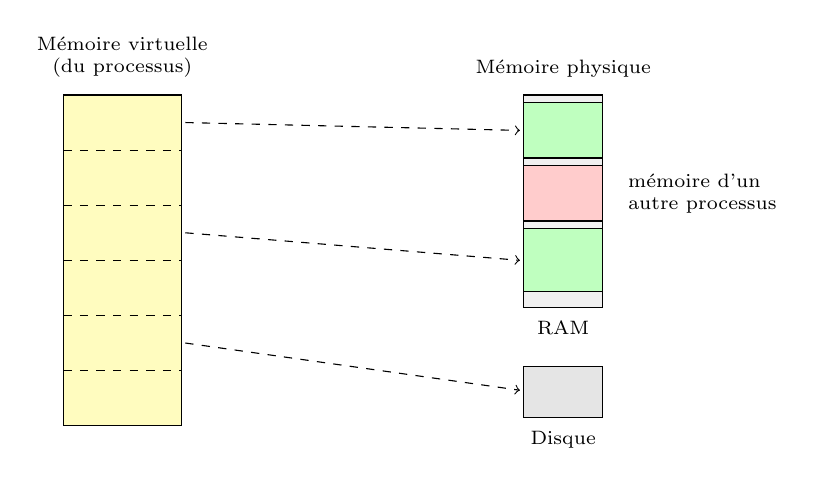
\begin{tikzpicture}[font=\small]
    \node[anchor=south, align=center, font=\scriptsize] at (1,4.3)
      {Mémoire virtuelle\\ (du processus)};
    \draw[fill=yellow!25] (0.25,0) rectangle (1.75,4.2);
    \foreach \y in {0.7,1.4,2.1,2.8,3.5} { \draw[dashed] (0.25,\y) -- (1.75,\y); }

    \node[anchor=south, align=center, font=\scriptsize] at (6.6,4.3) {Mémoire physique};
    \draw[fill=gray!12] (6.1,1.5) rectangle (7.1,4.2);
    \draw[fill=green!25] (6.1,3.4) rectangle (7.1,4.1);
    \draw[fill=red!20]   (6.1,2.6) rectangle (7.1,3.3);
    \draw[fill=green!25] (6.1,1.7) rectangle (7.1,2.5);
    \node[anchor=west, font=\scriptsize, align=left] at (7.3,2.95)
      {mémoire d'un\\ autre processus};
    \node[anchor=north, font=\scriptsize] at (6.6,1.45) {RAM};

    \draw[fill=gray!20] (6.1,0.1) rectangle (7.1,0.75);
    \node[anchor=north, font=\scriptsize] at (6.6,0.05) {Disque};

    \draw[->, dashed] (1.8,3.85) -- (6.05,3.75);
    \draw[->, dashed] (1.8,2.45) -- (6.05,2.1);
    \draw[->, dashed] (1.8,1.05) -- (6.05,0.45);
  \end{tikzpicture}
\end{figure}

\subsection{Programmation en GAS}
\paragraph{Définir des sections en GAS} Based on the mémoire virtuelle of the
processus, we may hence define the sections in which our data lives:
\begin{lstlisting}[language=gas]
        .text # debut d'une section de code
# ce qui est defini ici (donnees ou instructions) est executable

        .data # section de donnees modifiables
# ce qui est defini ici est modifiable mais n'est pas executable
.quad 0x1234567890 # la section commence par
      # 8 octets contenant le nombre 0x1234567890
      # qui prend minimum 5 octets a etre stocke
.byte 0x12 ; ces 8 octets sont suivi par un octet contenant
      ; 0x12 (=18 en decimal)
.ascii "Hello " ; H, e, l, l, o, ' '
.asciz "World" ; 6 octets W, o, r, l, d, \0
.helloworld: ; un label, une maniere d'adresser
        .string        "Hello World!\n" # la meme chose que asciz, donc 13+1=14 octets

        .bss # section de donnees modifiables initialisees a 0

        .text         # une autre section de code
        .globl _start # on veut exporter ce symbole
_start: # le label main correspondra a une function
        movq $42, .x(%rip)
        ret

# GCC rale si on ne finit pas par une speciale section protegee
.section        .note.GNU-stack,"",@progbits
\end{lstlisting}

\begin{remark}
  The trailing \verb|.note.GNU-stack| is required for the linker in \verb|gcc|
  to be able to certify that the program does not want an executable pile.
\end{remark}

\subsubsection{Registres et constantes, accès à la RAM}
In GAS,
\begin{itemize}
  \item on préfixe les registres par \verb|%| --- \verb|%rip|, \verb|%rbx|, etc.;
  \item on préfixe les nombres par \verb|$| --- \verb|$42|, \verb|$0x2A|, etc.
\end{itemize}
Plus généralement, \verb|offset(base, index, scale)| accède à
\[
  \text{offset} + v(\text{base}) + v(\text{index}) \times \text{scale},
\]
avec \textit{offset} en constante 32 bits signés, \textit{base} un registre,
\textit{index} un registre, \textit{scale} un entier parmi
$1, 2, 4, 8$. Any of the four parts may be omitted. On peut lire ou écrire
$1$, $2$, $4$ ou $8$ octets consécutifs.

\begin{center}
  \begin{tabular}{l l}
    \toprule
    Operand & Cell addressed \\
    \midrule
    \verb|(%rsp)|            & la case à la valeur de \verb|%rsp| \\
    \verb|4(%rsp)|           & la case à la valeur de $4 + $ \verb|%rsp| \\
    \verb|4(%rsp,%rdi,2)|    & la case à la valeur de $4 + $ \verb|%rsp| $+\, 2 \times$ \verb|%rdi| \\
    \verb|x(%rip)|           & the cell at the label \verb|x| (see below) \\
    \bottomrule
  \end{tabular}
\end{center}

\paragraph{Labels et multisections} Un registre spécial (\text{\%rip} en
x86-64) stocke l'adresse de l'instruction courante. Labels store
addresses relative to \text{\%rip}, so that the code can be
position-independent. We may hence use labels to obtain the address of a stored
variable:

\begin{lstlisting}[language=gas]
        .text
.globl _start # marque que le symbole _start sera visible
_start:       # dans le fichier ELF produit
      # differents adressages
      mov x(%rip), %rax # relatif
      lea x(%rip), %rcx # adresse
      ### toujours mettre label(%rip) pour parler de la valeur
      # a la position du label
# on n'est pas oblige de changer de section
# pour stocker notre nombre
x: .quad 0x1234567890
\end{lstlisting}

\begin{example}[Copying Data]
La copie de données se fait avec \verb|mov source destination| où \verb|source| et
\verb|destination| peuvent être :
\begin{itemize}
  \item un nombre comme \verb|$42| (décimal) ou \verb|0x2A| en hexadécimal;
  \item un registre \verb|%rbx|;
  \item une case mémoire \verb|(%rsp)|, \verb|4(%rsp)|, \verb|18(%rsp,%rax,4)|,
    \verb|x(%rip)|.
\end{itemize}
\begin{remark}
On peut spécifier le nombre d'octets à copier. It is specified with the suffixes
\verb|b|, \verb|w|, \verb|l| and \verb|q| for $1$, $2$, $4$ and $8$ bytes,
respectively. L'assembleur tente de deviner le nombre d'octets à copier mais ce
n'est pas toujours possible, p.~ex.\ \verb|mov $42, (%rsp)|. When the suffix is
omitted the guess is made from the operands, and there it fails because neither
operand carries a width. Toutes les combinaisons source/destination ne sont pas
possibles. Memory to memory copies, for instance, are not allowed, so
\verb|mov (%rsp),(%rax)| is illegal.
\end{remark}
\end{example}

\begin{lstlisting}[language=gas]
mov $42, %rax
mov helloworld(%rip), %rsi
mov $42, %eax
mov $42, %ax
mov $42, %al
movb $0x12, (%rax) ; ecrit un seul octet (byte)
movw $0x1234, (%rax) ; ecrit un mot (2 O)
movl $0x12345678, (%rax) ; ecrit mot long (4 O)
movq $0x12345678, (%rax) ; ecrit un quad (8 O)
                         ; en utilisant un 32 bits signe
movq $0x4883ec08, 4(%rip)
\end{lstlisting}

\subsubsection{Casting}
Extending a value from a smaller width to a larger one is called
\textbf{casting}. In x86-64, the choice between the two forms is the choice of
how the new high bits are filled.

\begin{example}[Casting]
  \verb|movq $0x12345678, (%rax)| writes \verb|0x0000000012345678|, while
  \verb|movq $0xFFFFFFFF, (%rax)| writes \verb|0xFFFFFFFFFFFFFFFF|, since
  the immediate is encoded as a signed 32-bit value and sign-extended to
  64 bits.
\end{example}

We may hence specify the extension from a source width to a destination width
with zero- or sign-extension:
\begin{lstlisting}[language=gas]
movzbl %al, %ecx ; extension with Zero
movswq %ax , %rcx ; extension Signed:
                  ; 1 if starts with 1, 0 otherwise
\end{lstlisting}

\begin{example}[C to Assembly]
  We then have the following example of a C program and its translation to assembly, obtained
  with \verb|gcc -S -O0|. Note that an \verb|int| is four bytes, so we use \verb|movl| and
  store it in a \verb|.long|; the \verb|pushq %rbp| / \verb|movq %rsp, %rbp| /
  \verb|popq %rbp| trio is the function prologue and epilogue; and the valeur de
  retour of \verb|main| is stored in \verb|%eax|.
  \begin{multicols}{2}
    \begin{lstlisting}[language=C]
    int x = 0x12;   // 18
    int main() {
      x = 0x34;     // 52
      x = 0x56;     // 86
      x = 0x78;     // 120
    }
    \end{lstlisting}\vfill\null
    
    \begin{lstlisting}[language=gas]
            .globl  x
            .data
    x:      .long   18
            .text
            .globl  main
    main:
            pushq   %rbp
            movq    %rsp, %rbp
            movl    $52, x(%rip)
            movl    $86, x(%rip)
            movl    $120, x(%rip)
            movl    $0, %eax
            popq    %rbp
            ret
    \end{lstlisting}
  \end{multicols}
\end{example}

\begin{example}[Disassembly]
  Below is the disassembly of the previous example. Utilisation de
  \verb|objdump -S| pour le \verb|main| et \verb|-d| pour le data.
  \begin{lstlisting}
  0000000000001129 <main>:
    1129: 55                      push %rbp
    112a: 48 89 e5                mov %rsp,%rbp
    112d: c7 05 d9 2e 00 00 34    movl $0x34,0x2ed9(%rip) # 4010 <x>
    1134: 00 00 00
    1137: c7 05 cf 2e 00 00 56    movl $0x56,0x2ecf(%rip) # 4010 <x>
    113e: 00 00 00
    1141: c7 05 c5 2e 00 00 78    movl $0x78,0x2ec5(%rip) # 4010 <x>
    1148: 00 00 00
    114b: b8 00 00 00 00          mov $0x0,%eax
    1150: 5d                      pop %rbp
    1151: c3                      ret
  .....
  Contents of section .data:
   4000 00000000 00000000 08400000 00000000 .........@......
   4010 12000000                            ....
  \end{lstlisting}
\end{example}
\begin{remark}
  Instructions are variable-length on x86-64. The three \verb|movl| stores
  each occupy ten bytes while \verb|ret| occupies one. 
\end{remark}

\subsubsection{Arithmétique}
\begin{lstlisting}[language=gas]
add $42, %rax ; %rax += 42
add $-4, %rsp ; %rsp += -4
add %rax, %rbx ; %rbx += %rax
sub %rax, %rbx ; %rbx -= %rax
inc %rbx ; %rbx++
incq (%rsp) ; interpret the 8 byte at positions %rsp
decq (%rsp) ; as an integer and inc/dec them
cmp %rax, %rbx ; compute the diff but stores nothing
\end{lstlisting}
\begin{lstlisting}[language=gas]
imul $42, %rax ; %rax *= 42
imul %rbx ; %rax = (%rax * %rbx) mod 2^64
          ; %rdx = (%rax * %rbx) / 2^64
          ; or %rax:%rdx = (%rax * %rbx)
          ; as signed 128 bits int
mul %rbx ; %rax:%rdx = %rbx * %rax unsigned

idiv %rbx ; %rax = computes %rax + 2^64 x %rdx / %rbx
          ; %rdx is the remainder % %rbx
          ; idivq segfaults if the result does not fit

lea -8(%rsp, %rdx,4), %rax ; %rax = -8+%rsp+%rdx*4
      ; usually used to compute addresses
\end{lstlisting}

The one-operand forms are implicit in \verb|%rax| and \verb|%rdx|. For division
the dividend is the 128-bit quantity \verb|%rdx:%rax|:
\[
  \texttt{\%rax} \seteq
    \myfloor{\frac{2^{64}\,\texttt{\%rdx} + \texttt{\%rax}}{\texttt{\%rbx}}},
  \qquad
  \texttt{\%rdx} \seteq
    \left(2^{64}\,\texttt{\%rdx} + \texttt{\%rax}\right) \mod \texttt{\%rbx}.
\]

\subsubsection{Manipulation Bit-À-Bit}
\begin{lstlisting}[language=gas]
not %rax ; reverse all bits
xor %rax, %rbx ; %rbx ^= %rax
or %rax, %rbx ; %rbx |= %rax
and %rax, %rbx ; %rbx &= %rax

sal $42, %rax ; Shift arithmetic left
sar $42, %rax ; Shift arithmetic right
shr $42, %rax ; Shift (logic) right

test %rax, %rbx ; computes & but stores nothing
\end{lstlisting}

\subsubsection{Sauts}
\begin{lstlisting}[language=gas]
jmp main ; go to main, do not put (%rip) here
jmp *%rax ; go to the address pointed by %rax
\end{lstlisting}

A jump target is a label written bare --- \emph{not} \verb|main(%rip)|, because
the operand of a jump already is an address rather than the contents of one.
The starred form \verb|jmp *%rax| is the indirect jump, and it is what function
pointeurs, \verb|switch| tables and virtual dispatch all compile to.

\subsubsection{Drapeaux Utiles}
Il existe un \textbf{registre de drapeaux} (\textit{flags register}) spécial, on
y retrouve les drapeaux suivants :
\begin{center}
  \begin{tabular}{c c l l}
    \toprule
    Bit & Abréviation & Nom & Description \\
    \midrule
    0  & CF & Carry Flag    & retenue ? (was there a carry?) \\
    2  & PF & Parity Flag   & pair ou impair ? (even or odd?) \\
    6  & ZF & Zero Flag     & nul ? (is it zero?) \\
    7  & SF & Sign Flag     & strictement négatif ? (strictly negative?) \\
    11 & OF & Overflow Flag & le calcul signé a débordé ? (did the signed computation overflow?) \\
    \bottomrule
  \end{tabular}
\end{center}

\subsubsection{Instructions Conditionnelles}
\begin{lstlisting}[language=gas]
jCOND fact ; jump on COND
cmovCOND %rbx, %rcx ; mov on COND
setCOND %rax ; set %rax to 1 when COND
             ; and to 0 otherwise
\end{lstlisting}

Every condition is invertible by inserting \verb|n|, so \verb|jne| is the
negation of \verb|je|, \verb|cmovnz| of \verb|cmovz|, and so on. Quelques
conditions usuelles :

\begin{center}
  \begin{tabular}{l l @{\qquad\qquad} l l}
    \toprule
    \verb|e|  & equal                     & \verb|ae| & above or equal / unsigned \\
    \verb|z|  & zero (same as above)      & \verb|g|  & greater / signed \\
    \verb|ge| & greater equal             & \verb|l|  & less / signed \\
    \verb|b|  & below / unsigned          & \verb|ge| & greater or equal / signed \\
    \verb|a|  & above / unsigned          & \verb|le| & less or equal / signed \\
    \verb|be| & below or equal / unsigned & \verb|p|  & parity is even \\
    \bottomrule
  \end{tabular}
\end{center}

\subsubsection{Interaction avec l'OS}
En x86-64, c'est la commande \verb|syscall| qui rend la main à
l'OS. The syscall number goes in \verb|%rax| and the arguments in \verb|%rdi|,
\verb|%rsi|, \verb|%rdx| (and then \verb|%r10|, \verb|%r8|, \verb|%r9|).

\begin{center}
  \begin{tabular}{c l c c c}
    \toprule
    \verb|%rax| & Nom & \verb|%rdi| & \verb|%rsi| & \verb|%rdx| \\
    \midrule
    0  & Read  & \verb|fd|    & \verb|char*| & \verb|count| \\
    1  & Write & \verb|fd|    & \verb|char*| & \verb|count| \\
    12 & Break & \verb|brk|   &              &              \\
    60 & Exit  & \verb|error| &              &              \\
    \bottomrule
  \end{tabular}
\end{center}

\begin{remark}
  En Linux tout est fichier notamment l'entrée, la sortie et la sortie d'erreur
  avec les \textbf{descripteurs de fichiers} (\textit{file descriptors},
  \verb|fd|) $0$, $1$, et $2$. On désigne par \verb|fd| $0$ la entrée standard,
  et par \verb|fd| $1$ la sortie standard.
\end{remark}

\subsection{Exercices: Programmation en GAS}

\begin{problem}[A program that does nothing]
\begin{lstlisting}[language=gas]
        .globl _start
_start:
        mov $60, %rax ; id of the syscall
        xor %rdi, %rdi ; a trick to set %rdi to 0
        syscall

        .section .note.GNU-stack ; pour gcc
\end{lstlisting}
\end{problem}

\begin{remark}
  The \verb|syscall| instruction is required to terminate the program,
  otherwise the CPU will continue executing off into whatever bytes follow.
\end{remark}

\begin{problem}[Hello World]
  Pour l'appel \verb|Write| il faut \verb|%rax| $= 1$; la chaîne a une longueur
  de $13$; et il faut un pointeur vers la chaîne dans \verb|%rsi|.  Pour avoir
  le pointeur, il faut que \verb|"Hello World!\n"| existe dans la mémoire; il
  faut trouver son adresse et la mettre dans \verb|%rsi|.
\begin{lstlisting}[language=gas]
        .data
helloWorld:
        .string "Hello World!\n"
        .text
        .globl _start
_start:
        lea helloWorld(%rip), %rsi ; load the address of the string
        mov $1, %rdi ; stdout = 1
        mov $13,%rdx ; size of string to be printed
        mov $1, %rax ; id of the syscall
        syscall
        mov $60, %rax
        xor %rdi, %rdi
        syscall
        .section .note.GNU-stack
\end{lstlisting}
\end{problem}

\begin{problem}[Hello World 10 times]
\begin{lstlisting}[language=gas]
_start:
        mov $10, %r8
.boucle:
        lea helloWorld(%rip), %rsi
        mov $1,        %rdi
        mov $13,%rdx
        mov $1, %rax
        syscall
        dec %r8
        jnz .boucle
        mov $60, %rax
        xor %rdi, %rdi
        syscall
        .section .note.GNU-stack
\end{lstlisting}
  On utilise \verb|dec| pour décrémenter et \verb|jnz| pour jump non zero. With
  these, a counter in \verb|%r8| turns the body into a loop.
\end{problem}

\begin{remark}
  Not all registres d'argument are preserved across a \verb|syscall|, and there
  is no guarantee that the kernel will not trash them, without knowing the
  implementation of the syscall.
\end{remark}

\subsubsection{Autres Exercices}
\begin{center}
  \begin{tabular}{l r}
    \toprule
    Consigne & Exemple \\
    \midrule
    afficher une ligne de \verb|'X'| & \verb|XXXXXX| \\
    afficher une pyramide de \verb|'O'| & \verb|OO| puis \verb|O| \\
    afficher une chaîne dont on ne connaît pas la longueur & \verb|Hello !| \\
    afficher un caractère stocké dans \verb|%r8| $(\dagger)$ & \verb|'c'| $= 99$ \\
    afficher en décimal petit-boutien l'entier dans \verb|%r8| & \verb|24| \\
    calculer $10!$ avec une boucle & \verb|3628800| \\
    \bottomrule
  \end{tabular}
\end{center}
